
%%% Local Variables: 
%%% mode: latex
%%% TeX-master: t
%%% End: 

\chapter{现有体系结构服务质量保障技术评估}
\label{chap:curarch}

%In todays new processors the number of cores is continuously increasing
%which in turn increase the number of threads or workloads that can 
%simultaneously be run. When multi-threaded
% applications run concurrently, they compete for shared
%resources including L3 cache.  At times, this L3 cache resource contention may 
%result in inefficient space utilization. For example a higher priority thread 
%may end up with lesser L3 cache resource or a cache sensitive app may not get
%optimal cache occupancy thereby degrading the performance.
%Cache Allocation kernel patch helps provides a framework for sharing L3 cache
% so that users can allocate the resource according to set requirements.

随着多线程技术与多核平台的发展,单个节点能够提供的越来越强大的计算资源,为硬件资源共享
提供了足够的支持;而虚拟化技术的发展,特别是新兴的容器技术的出现,更加促进了硬件资源
的共享。目前,主流互联网公司已经将其部分业务迁移到了虚拟化平台或容器平台中,
能过资源共享的方式提高服务器资源利用率,但如何进行有效的任务调度依然是一个待解决的问题。
这其中最关键的两点是:实时精准的性能监控和确定性的性能隔离。
基于这一需求现有的芯片厂商都提出了自己的解决方案, % 可能只有intel的方案
如大部分芯片都支持的Performance Counter功能,可以实时监控IPC、命中率、访存带宽等功能,
Intel在E5-v3系列CPU中更是提出了Resource Director Technology(RDT)技术,
增加的对末级缓存监控(CMT)和访存带宽的监控(MBM),以及末级缓存容量划分功能(CAT)。
本章的将对这些已有技术进行分析,并讨论如何将这些技术应用到数据中心系统中以实现服务质量
保障。
% 验证Loop-back的动态调速资源分配机制的有效性

\section{实验方法介绍}

\subsection{Benchmark与应用}

使用CloudSuite和BigDataBench,代替SPEC

Intel早在多年前便在Sandy Bridge处理器中加入Way-Based的Cache Partitioning技术,
并且由UC Berkeley对该处理器进行了分析对比试验,认为Cache Partitioning能在很多
情况下提升20\%的性能。
该工作主要面向SPEC负载,但数据中心中运行的应用与SPEC存在很大差别[][],
因此在本章,希望使用现有的服务质量保障技术,对数据中心应用混合,验证其效果。

我们将应用负载分为三类:(1) Guaranteed (2) Burstable (3) Best Effort。
其中第一类是最关键的应用,需要预留足够的资源以保证其性能,对外服务基本属于些类型,
典型包括延迟敏感型的应用(如WebServer、memcache等),XXXX; % 长时在线应用
第二类是次关键的应用,它的负载会随时间出现明显的波动性,因些其资源需求也存在波动,
典型的应用包括:XXXX; % 非关键业务
第三类主要指一些可被杀死并重启的批处理应用。 % 批处理业务

调度策略是保证第一类应用,并在其中穿插后两类应用以提高利用率;实时监控第一类应用
的性能变化,对其资源进行隔离;监控第二类应用的性能变化,在必要时杀死第三类应用。

在本章中,我们以XXX做为第一类应用的代表, % WebServer, Video Stream,性能必须严格保障
XXX做为第二类应用的代表,			% Cache Server, 性能可以降低在一定范围内
XXX做为第三类应用的代表,			% Hadoop
将其混合部署到同一台服务器,并能够保障第一类应用的服务质量,同时尽可能
的保证第二类应用的性能,并在空闲时间完成第三类应用。

\subsection{实验平台}

在学术界,提出很多方案,在体系结构层次上实现性能隔离,在第\ref{chap02:}章中我们讨论了
其中主要的方案,其中Cache容量划分对性能影响较大。
Intel早在多年前便在Sandy Bridge原型处理器中加入Way-Based的Cache Partitioning技术,
UC Berkeley通过对该处理器进行了分析对比试验,认为Cache Partitioning能在很多
情况下提升20\%的性能。
在最新的E5-v3系列CPU中,Intel正式加入了对Cache容量划分的支持,本章的实验全部采用该平台。

后面将首先将对Intel的CAT/CMT技术做一简要介绍,之后将介绍如何在这一平台上构建实验环境,
并对实验目标做详细说明。


%Cache Monitoring Technology and Cache Allocation Technology provide the hardware framework to manage a shared resource, like last level cache. As multithreaded and multicore platform architectures emerge, running workloads in single-threaded, multithreaded, or complex virtual machine environment, the last level cache is a key resource to manage. Intel introduces Cache Monitoring Technology and Cache Allocation Technology to manage these various workloads across shared resources.


%同时Intel的DDIO技术中也支持将LLC中的某几个Way分配给I/O数据,
%以减少I/O数据对其他应用程序的影响。华为海思的ARM处理器也提出一定的QoS技术,
%能对LLC进行按路划分;在内存控制器增加了控制机制。
%
%虽然这些处理器带有QoS功能,但在实际应用中却并没有得到广泛的应用。
%因此,本课题将主要验证上述QoS机制的有效场景与实际效果,
%同时验证带“Loop-back”的动态调整资源分配策略机制的有效性;
%并基于电信转发控制典型业务以及互联网媒体应用,分析时延约束,流量模型及噪音影响等,
%通过X86 QoS实测数据整理出QoS特性价值地图。

\subsubsection*{Intel Resource Director Technology(RDT)技术}

针对多处理器芯片中多应用共享的特征,Intel提出了Resource Director Technology方案来解决多应用资源共享冲突问题。
如图\ref{fig:intel-rdt-overview}所示,该方案的硬件基础是资源监控与资源分配控制机制,
同时提供基于"监控->策略->控制"组合的闭环方式来实现应用感知的资源管理框架。
其中资源监控提高了资源使用情况的能见度,使得资源利用率可以被跟踪,同时可以侦测到应用性能随资源的变化,
为上层的资源调度提供数据基础;
而硬件支持的资源分配控制机制,使得上层软件可以控制对硬件共享资源的使用。

% Intel RDT Overview
\begin{figure}[H]
  \centering
  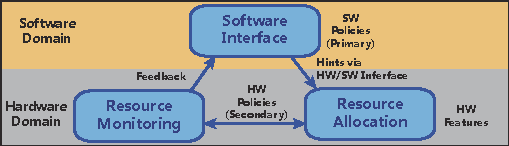
\includegraphics{x86eval/intel-rdt-overview}
  \caption[Intel Resource Director Technology (RDT) 技术示意图]{
    Intel Resource Director Technology (RDT)技术:硬件提供资源监控与分配功能,
    软件负责对资源使用进行调度,实现资源按需求动态分配。}
  \label{fig:intel-rdt-overview}
\end{figure}

目前Intel已经将RDT方案应用到共享末级缓存和内存控制器中,通过CMT/MBM技术实现对缓存容量
以及内存带宽的监控;通过CAT技术实现对缓存容量划分的支持。

CMT和MBM技术允许操作系统或Hypervisor/VMM监控在其上运行的应用对共享缓存与内存带宽
的使用情况,图\ref{fig:intel-cmt-flow}是该技术的流程示意图。
操作系统或VMM首先为执行实体(如线程、进程或虚拟机)分配资源编号RMID,后续的监控结果都将
以RMID的形式进行汇报。在OS/VMM执行调度并进行上下文切换时,将被调度实体的的RMID写入到目标
处理器核对应的寄存器中。OS/VMM可以随时通过RMID查询各个执行实体的资源使用情况,如共享缓存
占用或访存带宽等信息。
 
% Intel CMT Flow
\begin{figure}[H]
  \centering
  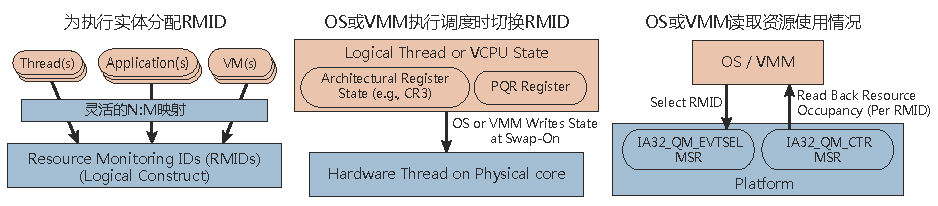
\includegraphics{x86eval/intel-cmt-flow}
  \caption[Intel Cache Monitor Technology (CMT) 技术流程]{Intel CMT技术流程:
   (1)为线程、应用或虚拟机等执行实体分配资源编号RMID;(2)将包含RMID的PQR寄存器
   保存在线程TCB或虚拟机VCPU中,并在执行上下文切换时写入到处理器核对应的物理寄存器中;
   (3)根据RMID使用MSRs寄存器获取共享资源使用情况。}
%Threads, applications, VMs or any combination can be associated with an RMID, enabling very flexible monitoring. As an example, all threads in a VM could be given the same RMID for simple per-VM monitoring. (2) The PQR register (containing an RMID) stored as part of a thread or VCPU state, which is written onto the thread-specific registers when a software thread is scheduled on a hardware thread for execution. (3) After a period of time (as defined by the software) the occupancy data for a given RMID can be read back through a pair of keyhole MSRs which provide the ability to input an RMID and Event ID (EvtID) in a selection MSR, and the hardware retrieves and returns the occupancy in the data MSR.}
  \label{fig:intel-cmt-flow}
\end{figure}

CAT技术为OS/VMM提供了控制末级共享缓存容量的功能,如图\ref{fig:intel-cat-flow}所示,
当该功能被开启后,应用将只能使用分配给它的Cache容量,实现路划分。
路划分策略是以COS为粒度进行指定,OS/VMM首先为某一COS制定路划分策略,并将该COS关联到使用
该策略的执行实体中,并在上下文划分时将被调度实体的COS写入到处理器核对应的寄存器中,
共享缓存根据COS对应的策略来进行缓存替换操作。

\begin{figure}[H]
  \centering
  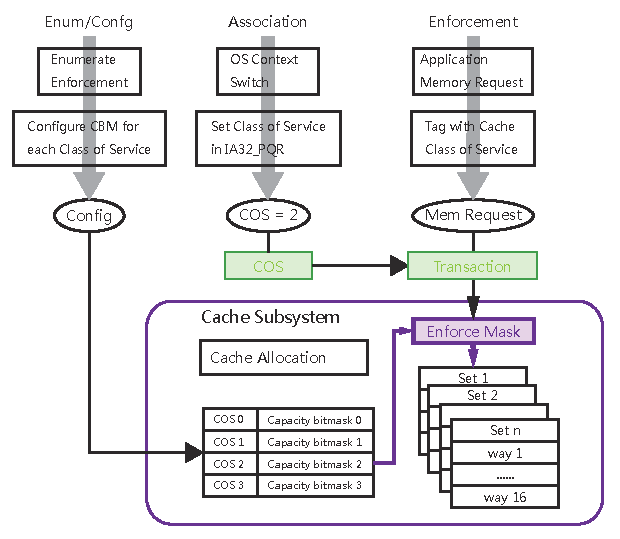
\includegraphics[height=8cm]{x86eval/intel-cat-flow}
  \caption[Intel Cache Allocation Technology (CAT) 技术流程]{Intel CAT技术流程}
  \label{fig:intel-cat-flow}
\end{figure}


\subsubsection*{ARM: Cache partition技术}

该部分需要更多的信息,如ARM64的支持。


\subsubsection*{实验平台组成}

本章所使用的实验平台由4台双路E5-v3服务器缓存,它们之间通过万兆以太网交换机互连,
如图\ref{}所示。
在该平台上部署了一个小型的Hadoop集群,HDFS配置为双副本,每个节点启用4个map和4个reduce任务;
在其上运行mahout/pagerank以及一些基于MapReduce的MicroBenchmark,做为离线应用。
同时在其中两个节点上配置了分布式的Cassandra做为分布式数据数据库实例,另外两个节点配置了
Nginx集群做为前端WebServer服务器,做为在线应用。


\section{共享缓存分析}

\subsection{缓存容量对性能影响}

递减Cache Way,对比性能,找出临界值

\subsection{缓存干扰对性能影响}

1. 运行两个应用,对比在线应用性能变化
2. 采用“限制离线应用缓存占用”策略
3. 采用“隔离在线离线应用缓存”策略

\subsection{小结}

\section{访存带宽分析}

\section{动态资源分配策略}

通过软件监控并设定阈值,对资源进行重新分配。包括Cache、CPU share等

设置不同的监控粒度,对比开销+性能变化



\section{本章小结}

通过本章研究,我们发现在没有体系结构支持的情况下,共享会存在很强烈的干扰现象,在使用
的软件隔离机制(cgroup)或调度机制后,可以在一定程度上缓解干扰。在传统体系结构下进行
扩展的新技术(如CMT/CAT),可以为共享提供一定的保障,但是需要OS或软件提供相应的支持,
因为我们需要一个新的体系结构来实现更好的服务质量保障。



